\subsection{Framework Consistency Assessment}

Our validation framework assesses both the precision (consistency across multiple runs) and accuracy (comparison with expert-created matrices) of the LLM-driven model construction process. This dual approach provides comprehensive insights into the framework's reliability and ecological validity.

We executed model generation across three distinct phases. In phase one, we established baseline configurations for each study region by processing species occurrence data and research parameters, creating standardized input states for subsequent iterations. In phase two, we executed five independent iterations per region, maintaining fixed input parameters while allowing the LLM's stochastic decision processes to generate natural variation in outputs. In phase three, we conducted detailed statistical analyses of both consistency across iterations and accuracy compared to expert-created matrices.

For consistency assessment, we calculated group stability scores using Jaccard similarity coefficients between consecutive iterations and analysed the coefficient of variation in diet proportions. For the accuracy assessment, we averaged the diet proportions of the five LLM-generated matrices and compared the resulting matrix with an expert-created matrix for the Great Australian Bight ecosystem (C. Bulman pers. comm.) that was used to inform \citep{Fulton2018}. 

\subsubsection{Study Regions}

\begin{figure}[htbp]
    \centering
    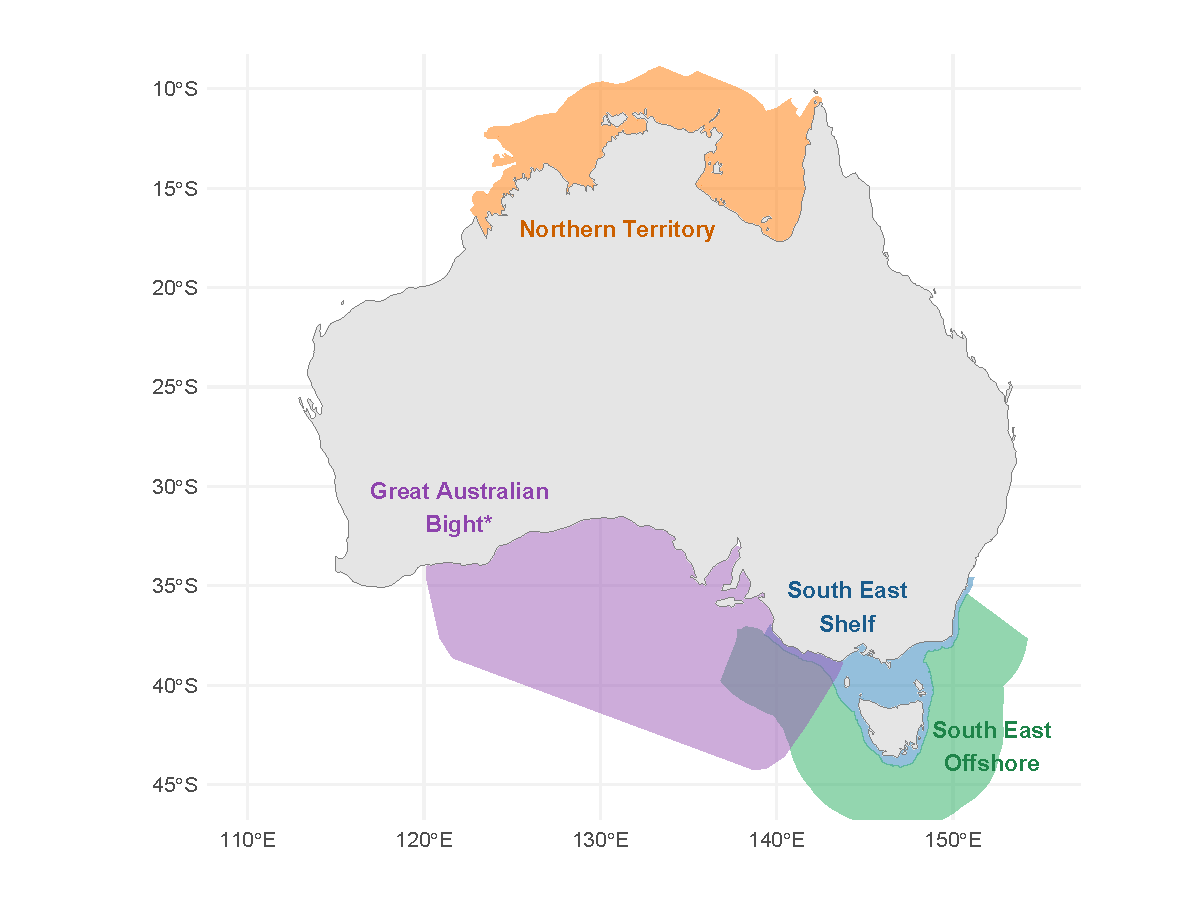
\includegraphics[width=0.8\textwidth]{figures/validation_regions.pdf}
    \caption{Map of the three study regions used for consistency assessment: Northern Territory (orange), South East shelf (blue), South East Offshore (green), and the Great Australian Bight (purple). *We used the GAB study region to test the accuracy of our approach by comparing it to the initial diet matrix used in \citep{Fulton2018}, we used the other regions to test the replicability of the approach.}
    \label{fig:validation_regions}
    \end{figure}

We assess our framework using three Australian marine regions that present distinct ecological characteristics and modelling challenges (Figure \ref{fig:validation_regions}). The Northern Territory region represents a tropical ecosystem characterised by complex reef systems, seasonal monsoon influences, and high biodiversity. This region tests the framework's ability to handle diverse species assemblages and complex trophic interactions in a dynamic environment.

The South East shelf region represents a temperate coastal system with extensive ecological records. This region has comprehensive diet information in established databases, well-documented EwE models spanning multiple years, and active research programs. The rich availability of expert knowledge and historical data makes this region ideal for assessing the framework's data integration capabilities.

The South East Offshore region presents a deep-water ecosystem that challenges the framework with data-limited conditions and unique ecological patterns. This region tests the framework's capacity to handle situations where direct observational data may be sparse and where species interactions may be less well understood. The contrasting characteristics of these three regions provide a robust test of the framework's adaptability across different ecological contexts.

\subsubsection{Species Grouping Reproducibility Analysis}

To assess the reproducibility of AI-generated species groupings, we developed quantitative measures of grouping consistency. We tracked each species' group assignments across iterations and calculated a consistency score:

\[
\text{Consistency Score} = \frac{\text{Number of occurrences in most common group}}{\text{Total number of iterations}}
\]

This metric quantifies the framework's decision-making reliability for individual species. We classified species with consistency scores below 0.95 as unstable, indicating variable group assignments across iterations. Chi-square tests on these consistency scores help identify whether grouping decisions remain stable across different ecological contexts, addressing a key aspect of the framework's reliability.

To evaluate broader patterns in group formation, we assessed group stability using the Jaccard similarity coefficient between consecutive iterations:

\[
J(i,j) = \frac{|M_{i} \cap M_{j}|}{|M_{i} \cup M_{j}|}
\]

where $M_{i}$ and $M_{j}$ represented species members in iterations $i$ and $j$. We calculated the overall stability score by averaging Jaccard similarities across consecutive iteration pairs. This approach, combined with coefficients of variation analysis, reveals how consistently the framework identifies and maintains ecologically meaningful groupings across different runs. One-way ANOVA tests on these stability measures across regions, supplemented with Cohen's f effect size calculations, demonstrate the framework's reproducibility across different marine ecosystems while maintaining consistent decision-making patterns.

\subsubsection{Diet Matrix Reproducibility Assessment}
To evaluate the consistency of AI-generated trophic interactions and assess the framework's ability to capture distinct ecological patterns, we developed a multi-metric analysis approach. We focused on significant predator-prey interactions, defined as those comprising more than 5\% of a predator's diet, using both descriptive statistics and correlation analyses. For each interaction, we calculated:

\begin{enumerate}
    \item Presence ratio across iterations:
    \[
    P_{ij} = \frac{\text{Number of iterations with interaction}}{n}
    \]
    where $n$ was the total number of iterations.

    \item Mean diet proportion:
    \[
    \mu_{ij} = \frac{1}{n}\sum_{k=1}^{n} x_{ijk}
    \]
    where $x_{ijk}$ represents diet proportion for predator $i$ consuming prey $j$ in iteration $k$.

    \item Stability score:
    \[
    S_{ij} = \frac{1}{n}\sum_{k=1}^{n} \frac{|x_{ijk} - \mu_{ij}|}{\max_{k}(x_{ijk})}
    \]
    where $x_{ijk}$ represents the diet proportion for predator $i$ consuming prey $j$ in iteration $k$, $\mu_{ij}$ is the mean diet proportion across iterations, and $\max_{k}(x_{ijk})$ is the maximum value across iterations. This score ranges from 0 (perfect stability) to 1 (maximum instability), with lower values indicating more consistent diet proportions across iterations.
\end{enumerate}

We chose this stability metric over traditional variance measures for several reasons. First, by normalizing deviations by the maximum value, the metric achieves scale independence, allowing meaningful comparisons between interactions of different magnitudes. For example, the sequences [0.2, 0.2, 0.2, 0.2, 0.1] and [0.02, 0.02, 0.02, 0.02, 0.01] would yield the same stability score despite having different absolute variances. Second, the bounded range between 0 and 1 provides an intuitive scale for assessing stability, unlike the unbounded nature of variance. Third, this approach effectively handles small variations in small values, ensuring that minor fluctuations in trace diet components do not disproportionately influence the stability assessment.

We classified interactions as unstable when their stability score exceeded 0.3, indicating significant variation in diet proportions across iterations. To illustrate this metric:

\begin{itemize}
    \item A stable interaction (S = 0.08) might show values [0.02, 0.02, 0.02, 0.02, 0.01], where proportions remain very similar across iterations
    \item An unstable interaction (S = 0.39) might show values [0.027, 0.25, 0.25, 0.067, 0.25], where proportions vary substantially between iterations
\end{itemize}

This metric provides a continuous measure of stability that handles both presence/absence patterns and magnitude variations in a unified way, avoiding discontinuities at zero values. To assess the framework's ability to capture distinct ecological patterns across regions, we employed pairwise Spearman correlations between iterations to evaluate the consistency of predator-prey relationships, focusing on significant interactions. This non-parametric approach accounts for the potentially non-normal distribution of diet proportions. We supplemented this with Kruskal-Wallis tests to identify significant differences in trophic structure across regions, providing evidence of the framework's ability to distinguish unique ecological characteristics in different marine ecosystems.

\subsubsection{Diet Matrix Accuracy Assessment}
\label{sec:accuracy_assessment}
To evaluate the accuracy of AI-generated diet matrices against expert knowledge, we conducted a detailed comparison using the Great Australian Bight (GAB) ecosystem model developed by \citet{Fulton2018}. We obtained the original, unbalanced diet matrix constructed by expert marine ecologists (C. Bulman, personal communication) and compared it with five independently generated AI matrices for the same region. We isolate the diet proportion accuracy by providing the AI system with the same list of groupings from the extant GAB model, thus testing the systems ability to sort species into the correct groups and then assign diet proportions according to those group. 

The analysis examined two fundamental aspects of the diet matrices: the structural patterns of predator-prey relationships and the quantitative diet proportions. We first assessed structural agreement by identifying matching and mismatching interactions between the expert and AI matrices. This binary presence-absence analysis yielded counts of concordant interactions, where both matrices agreed on the presence or absence of a feeding relationship, and discordant interactions where one matrix indicated a link while the other did not. We quantified the overall agreement using Cohen's Kappa coefficient, supplemented by true positive and negative rates to characterise the framework's ability to replicate expert-identified trophic relationships.

For predator-prey pairs where both matrices indicated an interaction, we conducted quantitative comparisons of the diet proportions. We calculated the Pearson correlation coefficients to measure the relationship between expert and AI-assigned proportions. We performed these analyses both at the whole-matrix level and for individual predator groups, enabling identification of systematic patterns in the framework's performance across different taxonomic groups.
